% Template for PLoS
% Version 3.1 February 2015
%
% To compile to pdf, run:
% latex plos.template
% bibtex plos.template
% latex plos.template
% latex plos.template
% dvipdf plos.template
%
% % % % % % % % % % % % % % % % % % % % % %
%
% -- IMPORTANT NOTE
%
% This template contains comments intended 
% to minimize problems and delays during our production 
% process. Please follow the template instructions
% whenever possible.
%
% % % % % % % % % % % % % % % % % % % % % % % 
%
% Once your paper is accepted for publication, 
% PLEASE REMOVE ALL TRACKED CHANGES in this file and leave only
% the final text of your manuscript.
%
% There are no restrictions on package use within the LaTeX files except that 
% no packages listed in the template may be deleted.
%
% Please do not include colors or graphics in the text.
%
% Please do not create a heading level below \subsection. For 3rd level headings, use \paragraph{}.
%
% % % % % % % % % % % % % % % % % % % % % % %
%
% -- FIGURES AND TABLES
%
% Please include tables/figure captions directly after the paragraph where they are first cited in the text.
%
% DO NOT INCLUDE GRAPHICS IN YOUR MANUSCRIPT
% - Figures should be uploaded separately from your manuscript file. 
% - Figures generated using LaTeX should be extracted and removed from the PDF before submission. 
% - Figures containing multiple panels/subfigures must be combined into one image file before submission.
% For figure citations, please use "Fig." instead of "Figure".
% See http://www.plosone.org/static/figureGuidelines for PLOS figure guidelines.
%
% Tables should be cell-based and may not contain:
% - tabs/spacing/line breaks within cells to alter layout or alignment
% - vertically-merged cells (no tabular environments within tabular environments, do not use \multirow)
% - colors, shading, or graphic objects
% See http://www.plosone.org/static/figureGuidelines#tables for table guidelines.
%
% For tables that exceed the width of the text column, use the adjustwidth environment as illustrated in the example table in text below.
%
% % % % % % % % % % % % % % % % % % % % % % % %
%
% -- EQUATIONS, MATH SYMBOLS, SUBSCRIPTS, AND SUPERSCRIPTS
%
% IMPORTANT
% Below are a few tips to help format your equations and other special characters according to our specifications. For more tips to help reduce the possibility of formatting errors during conversion, please see our LaTeX guidelines at http://www.plosone.org/static/latexGuidelines
%
% Please be sure to include all portions of an equation in the math environment.
%
% Do not include text that is not math in the math environment. For example, CO2 will be CO\textsubscript{2}.
%
% Please add line breaks to long display equations when possible in order to fit size of the column. 
%
% For inline equations, please do not include punctuation (commas, etc) within the math environment unless this is part of the equation.
%
% % % % % % % % % % % % % % % % % % % % % % % % 
%
% Please contact latex@plos.org with any questions.
%
% % % % % % % % % % % % % % % % % % % % % % % %

\documentclass[10pt,letterpaper]{article}
\usepackage[top=0.85in,left=2.75in,footskip=0.75in]{geometry}

% Use adjustwidth environment to exceed column width (see example table in text)
\usepackage{changepage}

% Use Unicode characters when possible
\usepackage[utf8]{inputenc}

% textcomp package and marvosym package for additional characters
\usepackage{textcomp,marvosym}

% fixltx2e package for \textsubscript
\usepackage{fixltx2e}

% amsmath and amssymb packages, useful for mathematical formulas and symbols
\usepackage{amsmath,amssymb}

% cite package, to clean up citations in the main text. Do not remove.
\usepackage{cite}

% Use nameref to cite supporting information files (see Supporting Information section for more info)
\usepackage{nameref,hyperref}

% line numbers
\usepackage[right]{lineno}

% ligatures disabled
\usepackage{microtype}
\DisableLigatures[f]{encoding = *, family = * }

% rotating package for sideways tables
\usepackage{rotating}

% Remove comment for double spacing
%\usepackage{setspace} 
%\doublespacing

% Text layout
\raggedright
\setlength{\parindent}{0.5cm}
\textwidth 5.25in 
\textheight 8.75in

% Bold the 'Figure #' in the caption and separate it from the title/caption with a period
% Captions will be left justified
\usepackage[aboveskip=1pt,labelfont=bf,labelsep=period,justification=raggedright,singlelinecheck=off]{caption}

% Use the PLoS provided BiBTeX style
\bibliographystyle{plos2015}

% Remove brackets from numbering in List of References
\makeatletter
\renewcommand{\@biblabel}[1]{\quad#1.}
\makeatother

% Leave date blank
\date{}

% Header and Footer with logo
\usepackage{lastpage,fancyhdr,graphicx}
\usepackage{epstopdf}
\pagestyle{myheadings}
\pagestyle{fancy}
\fancyhf{}
\lhead{\includegraphics[width=2.0in]{PLOS-Submission.eps}}
\rfoot{\thepage/\pageref{LastPage}}
\renewcommand{\footrule}{\hrule height 2pt \vspace{2mm}}
\fancyheadoffset[L]{2.25in}
\fancyfootoffset[L]{2.25in}
\lfoot{\sf PLOS}

%% Include all macros below

\newcommand{\lorem}{{\bf LOREM}}
\newcommand{\ipsum}{{\bf IPSUM}}

%% END MACROS SECTION


\begin{document}
\vspace*{0.35in}

% Title must be 250 characters or less.
% Please capitalize all terms in the title except conjunctions, prepositions, and articles.
\begin{flushleft}
{\Large
\textbf\newline{Interblink dynamics during various mental tasks}
}
\newline
% Insert author names, affiliations and corresponding author email (do not include titles, positions, or degrees).
\\
Temesgen Gebrehiwot\textsuperscript{1,\Yinyang},
Rafal Paprocki\textsuperscript{2,\Yinyang},
Artem Lenskiy\textsuperscript{3,*}{\textpilcrow}
\\
\bigskip
\bf{1} School of Electronics and Communication Engineering, Cheonan, South Korea
\\
\bigskip

% Insert additional author notes using the symbols described below. Insert symbol callouts after author names as necessary.
% 
% Remove or comment out the author notes below if they aren't used.
%
% Primary Equal Contribution Note
\Yinyang These authors contributed equally to this work.

% Additional Equal Contribution Note
% Also use this double-dagger symbol for special authorship notes, such as senior authorship.
\ddag These authors also contributed equally to this work.

% Current address notes
\textcurrency a Insert current address of first author with an address update
% \textcurrency b Insert current address of second author with an address update
% \textcurrency c Insert current address of third author with an address update

% Deceased author note
\dag Deceased

% Group/Consortium Author Note
\textpilcrow Membership list can be found in the Acknowledgments section.

% Use the asterisk to denote corresponding authorship and provide email address in note below.
* lensky@koreatech.ac.kr

\end{flushleft}
% Please keep the abstract below 300 words
\section*{Abstract}
In this paper we investigated how statistical properties of the blink rate variability changes during four mental tasks: resting, solving analytical problems, reading a passage and memory testing. To construct time series of inter-blink intervals (blink rate variability) we detected exact blink time in EEG recordings using our blink detection algorithm. We found that among 27 subjects, all subjects blinked less during reading session. Moreover, standard deviation of the blink rate variability is higher during reading. [HERE: MORE CONCLUSIONS FROM RESULTS] Thus, we conclude that the variability of inter-blink intervals decreases during tasks that require concentration and intense mental activity.



\linenumbers

\section*{Introduction}
Blinking is a semi-autonomic closing of the eyelids. Occurrence, reasons and characteristics of blink rate, varies between animals, and it is possible to trace the evolution of the blinking mechanisms through species. [1]. Every time we blink, our eyelids spread a cocktail of oils and mucous secretions across the surface of the eye to keep your globes from drying out. Each blink spreads the tears on the eye cornea to moisture and disinfects the eye. Reduced blink rate causes eye redness and dryness also known as Dry Eye, which belongs to the major symptoms of the Computer Vision Syndrome [2]. Besides blink keeps eyes protected against potentially damaging stimuli, such as bright lights and foreign bodies like dust. 
However, people don't even notice the world going into darkness every few seconds. The sudden changes in an image due to saccades or blinks, do not interfere with our subjective experience of continuity 3, the very act of blinking suppresses an activity in several areas of the brain responsible for detecting environmental changes, so that you experience the world as continuous. Researchers have shown the synchronous behavior in blinking between listener and speaker in face-to-face conversation [3]. 
The blinks have been known to be linked to interior brain activities. Ponder and Kennedy Z implicated that high processes are major determinants of Blink enhancements and inhibition [4]. 
Researchers have shown that blinks can play a significant role in detecting many different brain disorder and brain activities. Spontaneous Blink Rate (BR) has been studied in many neurological diseases like Parkinson's disease and Tourette syndrome [5-7]. Researchers have found that blink rates can be used as a source of data in detecting psychiatric disorders like schizophrenia and attention hyperactivity all this is because blinks are regarded as non-invasive peripheral markers of the central dopamine activity which makes their accurate detection more important. 
World Health Organization (WHO) has announced that the ninth cause of death globally is car accidents. National Motor Vehicle Crash Causation Survey (NMVCCS) has found that 30 percent of car accidents are caused by the drowsiness of drivers [13]. It is known that workload increases heart rate and heart rate are known to decrease in monotonous and drowsy conditions. On the other hand BR is inversely correlated with the increase of workload, so blinks can be used to detect drowsiness before accident happens [14].


It is evident that eye blinks in general and the BR specifically is linked to brain activity. In this paper, we investigate the relationship between brain activities during reading and memory test, and the blink rate variability. To estimate blink rate variability, we utilize a blink detection algorithm that we proposed earlier [8] and briefly describe in section 3. The experimental setup is described in section 2. In the sections 4 we discuss on the relationship between the blink rate and the task, and in section 5 we elaborate on the statistical properties of blink rate variability and their relationship to the reading task and memory test.    


% You may title this section "Methods" or "Models". 
% "Models" is not a valid title for PLoS ONE authors. However, PLoS ONE
% authors may use "Analysis" 
\section*{Materials and Methods}
\subsection*{Ethics statement}
All of the subjects provided written consent to the participation in experiment.
\subsection*{Subjects}
Twenty seven subjects (26 males and 1 female) have been recruited for the experiment. Subjects age varies from 20 to 45 years old. The subjects had no history of psychiatric illness, had normal physical, and they had not been affected by any significant medical, neurological or ophthalmological illness. To avoid substance abuse, we prepared a questionnaire testifying that they had none of these issues. Among them, five subjects were dropped due to heavy noise caused by the subjects falling asleep, adjusting the cap or constant head movements.  All of them were informed to participate in experiment only if they are not tired, hungry or stressed. They have received explanation about process of experiment, yet purpose had been undiscovered until after the experiment.

\subsection*{Experimental design}
The test for the data recording session consisted of five different stages: (A) 5 minutes of resting, (B) IQ test, (C) 5 minutes of resting again, (D)reading passage, and (E) comprehension test. We developed the testing software is such a way that it does not require any interventions from either the subjects or the experiment supervisor to conduct this experiment. The whole testing session took 30 minutes. The first 5 minutes is control resting stage. Then IQ test starts and continues for 10 minutes, asking subject to solve analytical problems. After that we have second, 5 minutes resting stage. Next one is the passage reading session. The passage takes 5 minutes and consists of basic facts about Ethiopia, and the target of this passage was to record data while subjects were trying to store memory. Lastly, subjects were given a 5 minutes comprehension test about the passage. The questions were derived from the information provided in the passage. It was designed to get subject to retrieve the memory they stored earlier making this session four different brain processes. To avoid tendency, for part of the subject we changed the order of the tests in such a way, that first they had break (A), then read passage (D), solve comprehension test (E), had second brake (C) and answer IQ quiz (B). Since EEG is prone to noise due to movement,  subjects were asked to sit comfortably and possibly still, with no hand movement, scratching nose and other unnecessary actions. In order to minimize movement, we made sure that subjects answered the question by using the numbers from 1 to 6 on the keypad of a keyboard. All questions and texts were displayed on one screen with no need to scroll or change pages. Width of the text has been narrowed to minimize horizontal eye movement. The subjects participating experiment were recorded with camera in order to confirm no one felt asleep.

\subsection*{Data acquisition and analysis}

The video stream while subjects were performing the test was captured with a Pointgrey Flea3 high frame rate USB camera. Video has been used to confirm subjects were no sleeping during experiment. Simultaneously, EEG signals were recorded using Mitsar-EEG 201 amplifier and accompanying WinEEG software. The electrodes were placed according to the international “10-20 system” standards of electrode placement [9]. Electro-gel was injected into electrodes hollow in order to decrease the electrode-skin resistance. Currently, we are more focused on the recording of the blinks than the brain data, but in the future we are planning to analyse EEG to detect different types of brain activities while performing these exams. We used bipolar montage while recording these signals, which means we determine the potential between Fp1 and Fp3, also Fp2 and Fp4 for both pairs. The recordings were then imported in the form of CSV files to Matlab for further analysis. The process of blink detection is described in our previous work [8].Blink rate variabilities for each of 5 sessions have been estimated from EEG signals.
(HERE: HOW DO WE ANALYSE BRV FOR STAGES?)


\begin{figure}[h]
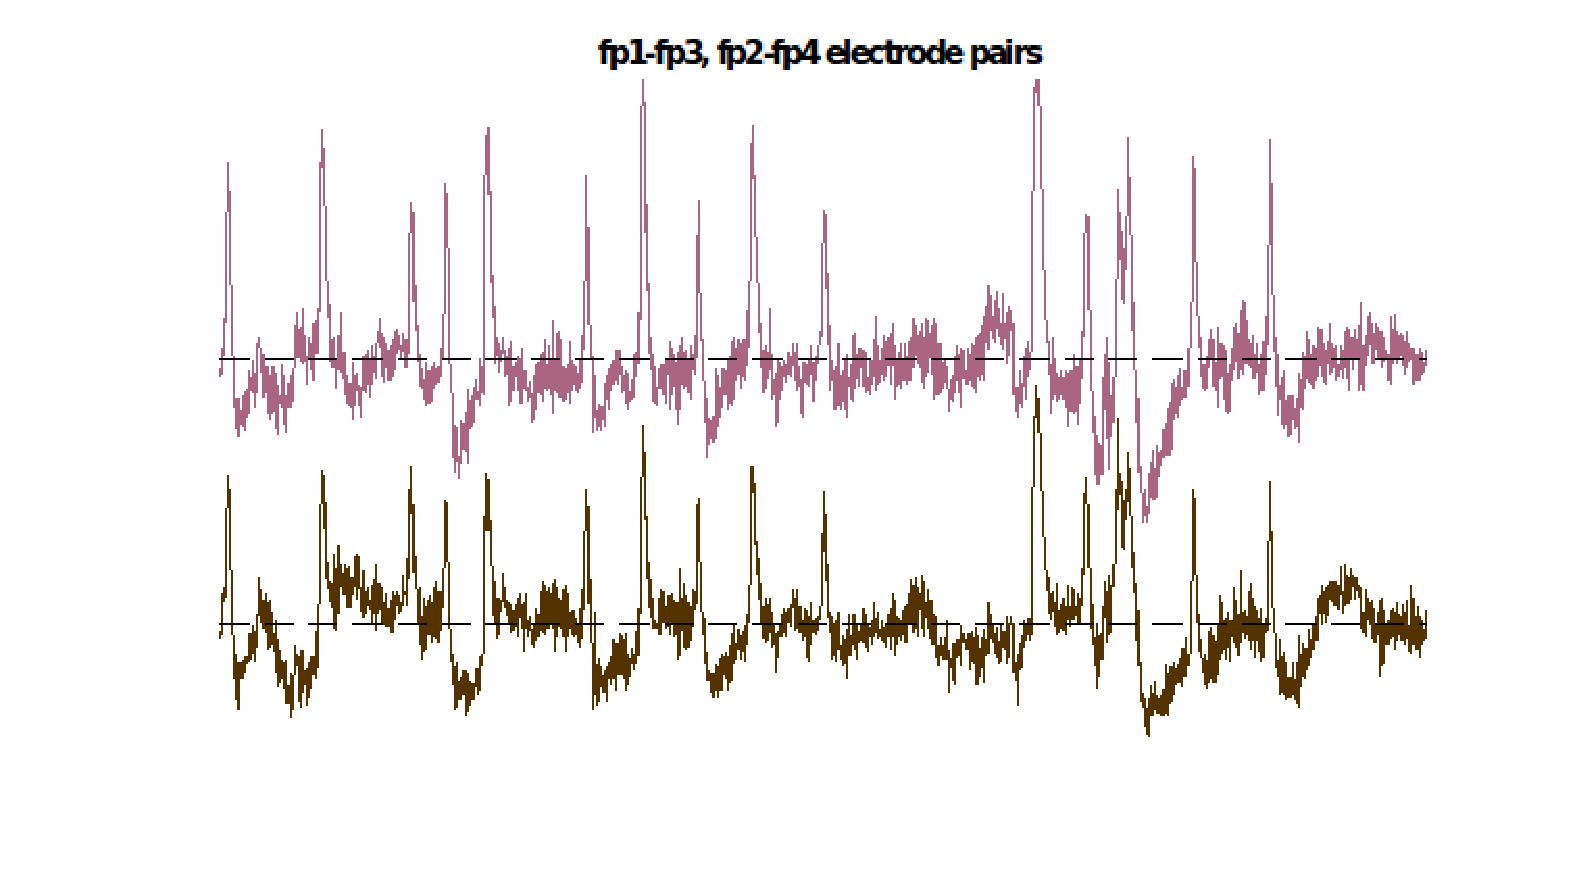
\includegraphics[width=5.0in]{img/signals.eps}
\caption{{\bf Figure Title first bold sentence Nulla mi mi, venenatis sed ipsum varius, volutpat euismod diam.}
Figure Caption Proin rutrum vel massa non gravida. Quisque tempor sem et dignissim rutrum. A: Lorem ipsum dolor sit amet. B: Consectetur adipiscing elit.}
\label{fig1}
\end{figure}

\begin{figure}[h]
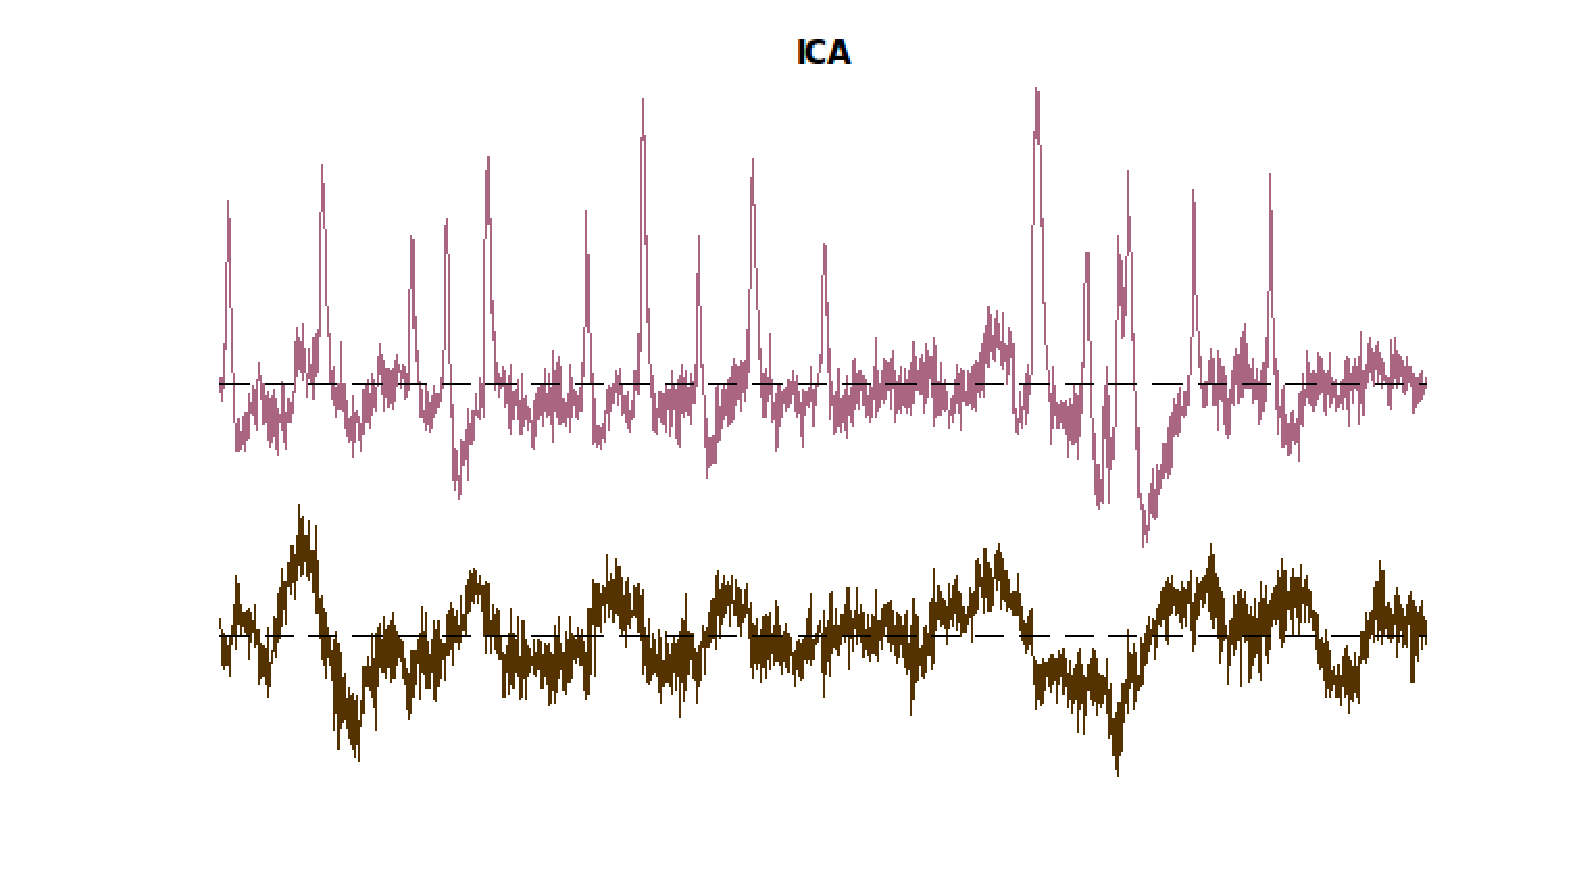
\includegraphics[width=5.0in]{img/components.eps}
\caption{{\bf Figure Title first bold sentence Nulla mi mi, venenatis sed ipsum varius, volutpat euismod diam.}
Figure Caption Proin rutrum vel massa non gravida. Quisque tempor sem et dignissim rutrum. A: Lorem ipsum dolor sit amet. B: Consectetur adipiscing elit.}
\label{fig2}
\end{figure}

\begin{enumerate}
\item{react}
\item{diffuse free particles}
\item{increment time by dt and go to 1}
\end{enumerate}

% Results and Discussion can be combined.
\section*{Results}


\subsection*{Relationship between interblink dynamics and mental tasks}
Bentivoglio et al, studied blink rate during rest, reading and conversation. It was showed that blink rate patterns are influenced more by cognitive processes rather than by age, eye color or gender [10]. Hart H.W distinguishes three types of an eye blink: spontaneous, reflex and voluntary were identified [11]. He also estimated that blinks occur on average, about 12 -15 times/min [11]. In [12] it was noted that spontaneous BR increases at the evening time. 
Here we investigate how the number of blinks changes depending on the task. We considered two tasks: reading a passage task and the memory test that is based on the same passage that subject was given. Among 13 subjects, all of them blinked less while reading. This result agrees with [15], where blinking has been related to certain cognitive processes. Blinking is a function of memory load, such that the more items in memory, the fewer the blinks.  Reading is an intensive process in which eyes moves quickly to assimilate text. It is necessary to understand that reading is a searching process intern this requires a prolonged focus on reading material as we are relating each words with its predecessors to make sense out of the whole sentence.
Operational memory, which is used during solving mental tasks, and visual imagination, may share components with a visual perceptual system. To avoid interference of cognitive processes, blinking is slowed down [16]. Number of blinks per each of 13 subjects is presented in table 1 and Fig.6. 
Fig. 7 and Fig. 8 compare BRV for all the subjects during the memory test. The X-axis is the blink interval where Y-axis presents interval lengths per each subject. Even though BRV visually looks different, the statistical properties are consistent. The mean and the standard deviations of BRV are lower during memory test than during reading session for all subjects. Passage test, as task involving memory, increases BR, while reading reduces it. Reading new information appears to be a heavier mental process than test, and operational memory is more in use. Moreover, in the text are longer, and ideas are more developed than in the test. Therefore, maybe we could find reflection in concept of blinking as an interlude between ideas or sentences[16]. 
Time between blinks changes, for reading it is shorter and elongates for the test. Fig. 9 presents average inter-blink per each subject in both stages, reading and memory test. Fig. 10 shows standard deviation of IBI dynamics.  Longer inter-blink in reading is caused because of fixation points while reading. Humans read each word at a time this are called fixation. From one fixation to another there is a search for the next fixation so this requires less blinks and more focus.  Also longer inter-Blinks are caused because reading is a cognitive process which increases brain activity [17].


\section*{Discussion}
In 1927 Ponder and Kennedy Z‘s implication that high processes are major determinants of blink enhancements and inhibition. They also mentioned that blinks might serve as an index of attention, or as they termed it “mental tension”. They inferred that person inhibits blinking while actively engaged in information abstraction, whether in response or to simple stimuli. In 1945, Hall wrote that blinks don’t occur randomly during reading.  
Our results have shown that there is lesser number of blinks in reading a passage than performing a memory test. Reading has lower blink rates because people read sentences by fixing on words so this search for the fixation will decrease there blinking rates. Also standard deviation of the blink rate variability is higher during reading. Studies suggested that blink behavior during reading is under perceptual and cognitive control [17].  Our results show higher blink rates while subjects performed the memory test. Subjects are aware that the memory test has a time limits and accessing memory needs faster brain activity. Therefore the conclusion is the inter-blink intervals’ variability decreases during tasks with more intensive workloads. In other words it means that task requires concentration and intense mental activity, when we start blinking rarely.


\section*{Supporting Information}

% Include only the SI item label in the subsection heading. Use the \nameref{label} command to cite SI items in the text.
\subsection*{S1 Video}
\label{S1_Video}
{\bf Bold the first sentence.}  Maecenas convallis mauris sit amet sem ultrices gravida. Etiam eget sapien nibh. Sed ac ipsum eget enim egestas ullamcorper nec euismod ligula. Curabitur fringilla pulvinar lectus consectetur pellentesque.

\subsection*{S1 Text}
\label{S1_Text}
{\bf Lorem Ipsum.} Maecenas convallis mauris sit amet sem ultrices gravida. Etiam eget sapien nibh. Sed ac ipsum eget enim egestas ullamcorper nec euismod ligula. Curabitur fringilla pulvinar lectus consectetur pellentesque.

\subsection*{S1 Fig}
\label{S1_Fig}
{\bf Lorem Ipsum.} Maecenas convallis mauris sit amet sem ultrices gravida. Etiam eget sapien nibh. Sed ac ipsum eget enim egestas ullamcorper nec euismod ligula. Curabitur fringilla pulvinar lectus consectetur pellentesque.

\subsection*{S2 Fig}
\label{S2_Fig}
{\bf Lorem Ipsum.} Maecenas convallis mauris sit amet sem ultrices gravida. Etiam eget sapien nibh. Sed ac ipsum eget enim egestas ullamcorper nec euismod ligula. Curabitur fringilla pulvinar lectus consectetur pellentesque.

\subsection*{S1 Table}
\label{S1_Table}
{\bf Lorem Ipsum.} Maecenas convallis mauris sit amet sem ultrices gravida. Etiam eget sapien nibh. Sed ac ipsum eget enim egestas ullamcorper nec euismod ligula. Curabitur fringilla pulvinar lectus consectetur pellentesque.

\section*{Acknowledgments}
Cras egestas velit mauris, eu mollis turpis pellentesque sit amet. Interdum et malesuada fames ac ante ipsum primis in faucibus. Nam id pretium nisi. Sed ac quam id nisi malesuada congue. Sed interdum aliquet augue, at pellentesque quam rhoncus vitae.

\nolinenumbers

%\section*{References}
% Either type in your references using
% \begin{thebibliography}{}
% \bibitem{}
% Text
% \end{thebibliography}
%
% OR
%
% Compile your BiBTeX database using our plos2015.bst
% style file and paste the contents of your .bbl file
% here.
% 
\begin{thebibliography}{10}
\bibitem{bib1}
Devaraju P, Gulati R, Antony PT, Mithun CB, Negi VS. Susceptibility to SLE in South Indian Tamils may be influenced by genetic selection pressure on TLR2 and TLR9 genes. Mol Immunol. 2014 Nov 22. pii: S0161-5890(14)00313-7. doi: 10.1016/j.molimm.2014.11.005

\bibitem{bib2}
Huynen MMTE, Martens P, Hilderlink HBM. The health impacts of globalisation: a conceptual framework. Global Health. 2005;1: 14. Available: http://www.globalizationandhealth.com/content/1/1/14.

\end{thebibliography}



\end{document}

